\chapter{Demands of an Energy Cluster}
\label{ch:background}
\par An \textbf{Energy Cluster} is a group of institutions, businesses, and individual customers working to produce, exchange, and distribute electrical energy. These clusters allow smaller agents in the energy market to cooperate and pool their resources to make their energy infrastructure safer, more efficient, and more profitable. This arrangement allows these entities to get more favorable deals when buying and selling electricity back to the grid \citep{UwarunkowaniaRozwojuEnergetykiRozproszonej}. 
\par Energy clusters typically include mid-sized enterprises and smaller individual energy plants, but they can also include larger institutions dedicated solely to generating electricity. 
\par Energy clusters also help to promote the development of renewable energy sources, such as solar, wind, and hydroelectric \citep{UwarunkowaniaRozwojuEnergetykiRozproszonej}.

\section{Historical and legal background} 

\par Fossil fuels, mainly coal, play a crucial role in Polish energy production. Most energy-producing coal plants were built in the waning decades of the previous century. Since then, renewable energy has been on the constant rise, especially solar technologies, which saw a sudden growth in 2020 thanks to the influx of prosumers - entities simultaneously producing and consuming energy \citep{CarbonPoland} \citep{Prosumer}.
\par Five large governmental entities dominate the Polish energy distribution market, each operating in its distribution area. These large distribution network operators (or DNO) are, in order of their size \citep{dostawcyPradu}:
\begin{itemize}
  \item Tauron Dystrybucja S.A.
  \item PGE Dystrybucja S.A.
  \item ENERGA-OPERATOR SA.
  \item Enea S.A.
  \item E.ON Polska S.A. (formerly innogy Polska S.A.)
\end{itemize}
\begin{figure}[htbp]
 \centering
 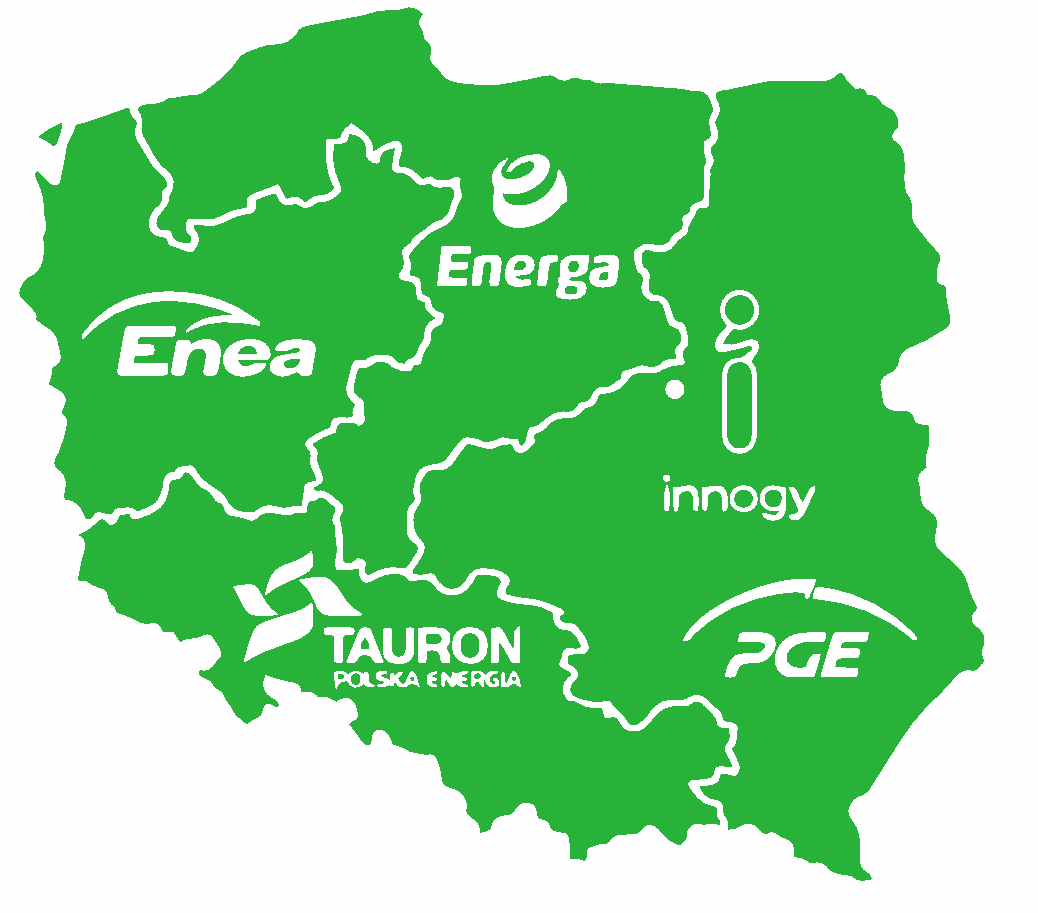
\includegraphics[width=0.5\textwidth]{gfx/EnergyDistributionMap}
 \caption{Distribution Network Operators in Poland \citep{mapkaEprad}}
 \label{fig:chapter02:energydistribution}
\end{figure}
\par Energy Clusters introduce a local alternative to these large enterprises. 
\par The Polish Law defines an energy cluster as ''Cywilnoprawne porozumienie, w skład którego mogą wchodzić osoby fizyczne, osoby prawne, jednostki naukowe, instytuty badawcze lub jednostki samorządu terytorialnego, dotyczące wytwarzania i równoważenia zapotrzebowania, dystrybucji lub obrotu energią z odnawialnych źródeł energii lub z innych źródeł lub paliw, w ramach sieci dystrybucyjnej o napięciu znamionowym niższym niż 110 kV, na obszarze działania tego klastra nieprzekraczającym granic jednego powiatu lub 5 gmin. Obszar działania klastra energii ustala się na podstawie miejsc przyłączenia wytwórców i odbiorców energii będących członkami tego klastra.'' [A Civil law agreement, between natural persons, legal persons, research institutions or local governments, on production, exchange, distribution or turnover of energy from renewable energy sources, or other sources or fuels, as a part of a distribution network with rated voltage lower than 110 kV, and an operational area lower than one county or five municipalities. The energy cluster's operational area is defined, based on the locations of energy producers and consumers, belonging to that energy cluster.]  (art. 2 p. 15a Act on Renewable Energy Sources) \citep{RESAct}.
\par These Energy clusters are represented by an Energy Cluster Coordinator, defined by polish law as ''Spółdzielnia, stowarzyszenie, fundacja, wskazane w porozumieniu cywilnoprawnym lub dowolny członek klastra energii, powołany w celu reprezentowania klastra'' [A cooperative, assocation, foundation, mentioned by a civil law agreement, or any energy cluster member, obligated to represent the cluster] (art. 2 p. 15a Act on Renewable Energy Sources)\citep{RESAct}.
\par Energy clusters are thus not an entity onto themself but an accord that defines its participants, operational area, its representative in the form of the coordinator, and its purpose and activities, whether that be production, distribution, sale, or storage of energy. It should also define the rights and responsibilities of every cluster member, the internal organization of the cluster, and how the agreement may be altered or dissolved \citep{ksiazka}.
\par One common type of an energy cluster member is the so-called prosumer, a portmanteau of producer and consumer. The RES act defines them as entities buying and producing energy from renewable sources for their own purposes \citep{Prosumer} \citep{RESAct}. 

\section{The functioning of energy clusters}

\par To establish a functioning energy cluster, its members should define a name and location of the cluster, list all of its members, and name one of them the coordinator, whose role is to manage the cluster and ensure work inside it goes smoothly \citep{ksiazka}.
\par The most apparent duty of energy clusters is to produce, exchange, and sometimes store electricity their members produce or buy from the outside grid. The necessary infrastructure can be either borrowed from the public grid upon a prior agreement or be explicitly built for the cluster.
\par Another essential responsibility of every cluster member is to measure how much energy each produces and consumes, along with the quality of said energy. These measurements are then analyzed to ensure compliance with the cluster agreement and national energy production and distribution laws \citep{ksiazka}.
\par The energy produced by clusters usually comes from renewable sources, although current law also allows some use of fossil fuels \citep{UwarunkowaniaRozwojuEnergetykiRozproszonej}.

\section{The Energy Cluster infrastructure}

\par The energy cluster members need to agree on the energy delivery method. These entities can exchange energy by using: 
\begin{enumerate}
  \item existing infrastructure,
  \item their private infrastructure, 
  \item a hybrid model consisting of the previous options.
\end{enumerate}
\par The most economical and popular option is to use the public energy grid. In such cases, the energy cluster coordinator has to apply with the appropriate DNO for access to the infrastructure, and the DNO is obligated to, whenever possible, connect every applying entity to the existing grid without prioritizing any other entity.
\par The less common option is to use a private energy grid explicitly made for the energy cluster. This method comes with responsibilities similar to those imposed on more traditional entities outside the energy cluster and much higher costs than using the public grid. It can, however, be economically sound in the case of many huge energy producers and consumers close to one another.

\section {Members of an energy cluster}

\par Various entities compose an energy cluster, some of which produce or consume energy, and others handle organizational matters. 
\par The public administration is frequently an initiator of such initiatives, especially given their benefits to the local economy and government funding provided for energy cluster development. It may help resolve conflicts of interests of competing cluster members or help procure necessary funding faster and more efficiently \citep {ksiazka}.
\par Some of the most vital members of energy clusters are local businesses. Their membership is mutually beneficial since while energy clusters can help their development, such enterprises provide the necessary funding and experience to build the clusters network faster.
\par The rest of the cluster membership constitutes prosumers with small energy-producing installations capable of satisfying at least some of their energy consumption \citep{ksiazka}.
\par Every energy cluster needs to choose, amongst its members, a coordinator to represent the cluster. It is usually a private company operating in the energy distribution market with the necessary funds and permits to produce and distribute energy. It can apply for any further permits needed in the future and take loans in the name of the cluster. Sometimes, that company acts exclusively as an energy cluster coordinator, efficiently managing the entire system \citep{ksiazka}.
\par The coordinator can also be an association of natural persons making up the energy cluster, a foundation comprising both natural and legal persons, a cooperative, or a company. It has to be a legal person, meaning entities such as partnerships or homeowner associations cannot in themselves be a part of an energy cluster \citep{ksiazka}.

\section{Energy meters}

\par Energy cluster members have to use energy meters to measure energy quality, consumption, and compliance with previously established norms. Data gathered by these meters is then used to improve efficiency, reduce costs, and optimize energy usage. They must be installed in every energy cluster member, whether a small prosumer or big industrial plant.
\par One example of an energy meter applicable in energy clusters and available on the market is the Otus 3 Three-phase electricity meter. Designed for residential use and capable of connecting to intelligent systems, it can gather and send to a database essential data about energy quality and its use by an energy cluster member \citep{otus}.
\par Optus 3's creators, the company Apator, in collaboration with Atende Industries, is in the process of creating an improved smart meter, specifically for the purposes of Energy Clusters and decentralized energy \citep{atende}.
\par Some of the most essential parameters gathered or checked against by meters such as Otus 3 include:
\begin{description}
  \item[The total energy produced/consumed] by energy cluster members is essential to monitor for two reasons: calculating an energy-produced-to-consumed balance that compares how much more or less energy was produced than consumed at any given window of time. Since excess energy is delivered to the energy cluster infrastructure to be consumed by other members or sold on the energy market, this balance has to be included in the energy settlement. Another reason to observe the total consumed energy is to monitor the exceedance of \textbf{contracted energy}. Contracted energy is the maximum amount of electrical energy an energy cluster member can consume at any given time. It should be specified in the energy cluster agreement based on the particular member's energy needs and the cluster's infrastructure capacity to provide said energy. Establishing a contracted amount of energy consumption with energy cluster members is a vital step in estimating the capacity of the cluster to satisfy all its members' needs. 
  \item[Reactive power] is the natural consequence of capacitance and inductance's presence in AC systems. When connected to an AC circuit, capacitors and inductors cause a phase shift between the voltage and current in the circuit. A phase shift in the form of reactive power, introduced to the grid, can cause instability and loads of other problems and thus is undesirable. Because capacitors cause a leading phase shift, while inductors cause a lagging one, these shifts can balance each other out; thus, maintaining a proper balance between capacitor-heavy and inductor-heavy devices is essential. A vector on the complex plane can be drawn, with real power drawn on the vertical axis and reactive power drawn on the horizontal axis. Such a vector in systems with leading reactive energy usually lands in the first quadrant of the plane, while lagging reactive energy usually results in the vector landing in the fourth quarter. An entity producing too much reactive energy in either direction has to pay fines per the energy cluster agreement. According to the decree of the Minister of Economy from 18th September 2011, the formula used to calculate the fine paid for excessive reactive energy produced is as follows /citep{rozpo}: $O_{b} = k \times C_{rk} \times (\sqrt{{{1 + tg^2 \varphi} \over {1 + tg^2 \varphi_{0}}} - 1}) \times A$ where:
\begin{itemize}
  \item $O_{b}$ is the fine paid for excessive reactive energy.
  \item $C_{rk}$ is the price of electrical energy, referred to in Article 23, paragraph 2 point 18, letter b of the law in force on the day of tariff approval.
  \item $k$ is the multiple of price $C_{rk}$ established in the tariff.
  \item $tg \varphi_{0}$ is a power factor established according to the decree.
  \item $tg \varphi$ is a power factor resulting from reactive power. It is equal to ${tg \varphi} = {{{\Delta E_{b}} \over A} + tg \varphi_{0}}$ where $\Delta E_{b}$ is the excess reactive energy recorded by a measuring device within the settlement period.
  \item $A$ is the active energy taken around the clock or for the time zone in which reactive energy consumption is controlled.
\end{itemize}
  \item[Frequency] is the number of cycles per second in an alternating current system, measured in hertz. It is vital to measure it since if the frequency of the electrical energy in an energy grid deviates significantly from the standard frequency, it can cause problems with the equipment connected to the grid, such as equipment operating too fast or causing significant wear. The energy grid operator has to ensure that frequency stays stable according to norms. An entity may monitor frequency to document cases of that duty not being fulfilled. According to the Power System Regulation, ''wartość średnia częstotliwości mierzonej przez 10 sekund w miejscach przyłączenia powinna być zawarta w przedziale: a) 50 Hz ± 1 \% (od 49,5 Hz do 50,5 Hz) przez 99,5\% tygodnia, b) 50 Hz + 4\% / -6\% (od 47 Hz do 52 Hz) przez 100\% tygodnia;'' [the average value of frequency measured in a period of 10 seconds in the point should be within the range of: a) 50 Hz ± 1 \% (from 49,5 Hz to 50,5 Hz) within 99,5\% of a week, b) 50 Hz + 4\% / -6\% (from 47 Hz to 52 Hz) within 100\% of a week] (Power System Regulation)\citep{psr}.
  \item[Voltage] is the measure of the flow of electrical current. It is another vital qualitative measure of electricity. Similarly to frequency, irregular electrical power voltage can slow down or even damage equipment and infrastructure, so it is vital to quickly monitor voltage to fix anomalies. The Power System Regulation Act, prescribes the following limits on allowed voltage: ''w każdym tygodniu 95\% ze zbioru 10-minutowych średnich wartości skutecznych napięcia zasilającego powinno mieścić się w przedziale odchyleń: a) ±10\% napięcia znamianowoego dla sieci o napięciu znamionowym 110V i 220V, b) +10\% / -10\% napięcia znamionowego dla sieci o napięciu znamionowym 400kV'' [within each week, 95\% of the sets of effective values of data gathered over 10 minutes, should be within the range of: a) ±10\% of rated voltage for an energy grid with rated voltage of 110V and 220V, b) +10\% / -10\% of rated voltage for an energy grid with rated voltage of 400kV] (Power System Regulation)\citep{psr}.
\end{description}

\section{Data structure}

\par Data gathered from meters is usually structured as pairs of data values and the time of measurement timestamps. Additional information, such as data acquisition to the database timestamp or the data's point of origin, may also be included, depending on the implementation. 
\par A sample series of data gathered from a particular energy meter over the year 2022 has been provided by the Energy Cluster in Ochotnica Dolna. Data in this set is first organized into separate metrics, described by rows of data, each containing\citep{ochotnica}:
\begin{enumerate}
  \item A timestamp, representing the time and date of data capture.
  \item A timestamp, representing the time and date of data acquisition into the database.
  \item A real number, representing the metric's value at the given point in time.
  \item An integer, representing an ID of the energy meter that provided the data.
\end{enumerate}

\begin{table}[!ht]
    \centering
    \caption{Energy consumed at one member of the Energy Cluster in Ochotnica Dolna \citep{ochotnica}}
    \begin{tabular}{llll}
    \hline
        "cap\_time (utc)" & "acq\_time (utc)" & "value" & "origin" \\ \hline
        "2021-09-14 10:30:00,000" & "2021-09-21 09:05:59,004" & "0.220" & 1 \\ 
        "2021-09-14 10:45:00,000" & "2021-09-21 09:05:59,472" & "1.804" & 1 \\ 
        "2021-09-14 11:00:00,000" & "2021-09-21 09:05:59,882" & "3.290" & 1 \\ 
        "2021-09-14 11:15:00,000" & "2021-09-21 09:06:00,406" & "4.654" & 1 \\ 
        "2021-09-14 11:30:00,000" & "2021-09-21 09:06:00,921" & "6.143" & 1 \\ 
        "2021-09-14 11:45:00,000" & "2021-09-21 09:06:01,346" & "7.667" & 1 \\ 
        "2021-09-14 12:00:00,000" & "2021-09-21 09:06:01,860" & "9.323" & 1 \\ 
        "2021-09-14 12:15:00,000" & "2021-09-21 09:06:02,284" & "10.817" & 1 \\ 
        "2021-09-14 12:30:00,000" & "2021-09-21 09:06:02,733" & "12.518" & 1 \\ 
        "2021-09-14 12:45:00,000" & "2021-09-21 09:06:03,144" & "14.196" & 1 \\ \hline
    \end{tabular}
\end{table}

\begin{table}[!ht]
    \centering
    \caption{Phase L1 voltage measured at one member of the Energy Cluster in Ochotnica Dolna \citep{ochotnica}}
    \begin{tabular}{llll}
    \hline
        "cap\_time (utc)" & "acq\_time (utc)" & "value" & "origin" \\ \hline
        "2021-09-21 09:12:41,000" & "2021-09-21 09:12:42,146" & "233.740" & 1 \\ 
        "2021-09-21 09:13:40,000" & "2021-09-21 09:13:41,992" & "231.355" & 1 \\ 
        "2021-09-21 09:14:40,000" & "2021-09-21 09:14:41,354" & "236.173" & 1 \\ 
        "2021-09-21 09:15:40,000" & "2021-09-21 09:15:41,299" & "229.385" & 1 \\ 
        "2021-09-21 09:16:39,000" & "2021-09-21 09:16:40,542" & "230.810" & 1 \\ 
        "2021-09-21 09:17:40,000" & "2021-09-21 09:17:41,683" & "227.255" & 1 \\ 
        "2021-09-21 09:18:39,000" & "2021-09-21 09:18:41,027" & "227.516" & 1 \\ 
        "2021-09-21 09:19:39,000" & "2021-09-21 09:19:41,054" & "227.345" & 1 \\ 
        "2021-09-21 09:20:39,000" & "2021-09-21 09:20:40,305" & "227.166" & 1 \\ 
        "2021-09-21 09:21:38,000" & "2021-09-21 09:21:39,634" & "232.959" & 1 \\ \hline
    \end{tabular}
\end{table}

\par Metrics captured by said meter include:
\begin{itemize}
  \item Energy provided to the energy grid [kV]
  \item Energy consumed from the energy grid [kV]
  \item Quarter 1 reactive energy [kVAr]
  \item Quarter 2 reactive energy [kVAr]
  \item Quarter 3 reactive energy [kVAr]
  \item Quarter 4 reactive energy [kVAr]
  \item Power line frequency [Hz]
  \item Phase 1 effective value of voltage [V]
  \item Phase 2 effective value of voltage [V]
  \item Phase 3 effective value of voltage [V]
\end{itemize}